%%%%%%%%%%%%%%%%%%%%%%%%%%%%%%%%%%%%%%%%%%%%%%%%%%%%%%%%%%%%%%%%%%%%%%%%%%%%%%%%
%2345678901234567890123456789012345678901234567890123456789012345678901234567890
%        1         2         3         4         5         6         7         8

\documentclass[letterpaper, 10 pt, conference]{ieeeconf}  % Comment this line out if you need a4paper

%\documentclass[a4paper, 10pt, conference]{ieeeconf}      % Use this line for a4 paper

\IEEEoverridecommandlockouts                              % This command is only needed if 
                                                          % you want to use the \thanks command

\overrideIEEEmargins                                      % Needed to meet printer requirements.

%In case you encounter the following error:
%Error 1010 The PDF file may be corrupt (unable to open PDF file) OR
%Error 1000 An error occurred while parsing a contents stream. Unable to analyze the PDF file.
%This is a known problem with pdfLaTeX conversion filter. The file cannot be opened with acrobat reader
%Please use one of the alternatives below to circumvent this error by uncommenting one or the other
%\pdfobjcompresslevel=0
%\pdfminorversion=4

% See the \addtolength command later in the file to balance the column lengths
% on the last page of the document

% The following packages can be found on http:\\www.ctan.org
\usepackage{graphics} % for pdf, bitmapped graphics files
\usepackage{epsfig} % for postscript graphics files
\usepackage{mathptmx} % assumes new font selection scheme installed
\usepackage{times} % assumes new font selection scheme installed
\usepackage{amsmath} % assumes amsmath package installed
\usepackage{amssymb}  % assumes amsmath package installed
\usepackage{mathtools}
\usepackage{relsize}
\usepackage{tikz}
\graphicspath{{./Drawings/}} 

\title{\LARGE \bf
Robustly constrained data-driven control
}


\author{Albert Author$^{1}$ and Bernard D. Researcher$^{2}$% <-this % stops a space
\thanks{*This work was not supported by any organization}% <-this % stops a space
\thanks{$^{1}$Albert Author is with Faculty of Electrical Engineering, Mathematics and Computer Science,
        University of Twente, 7500 AE Enschede, The Netherlands
        {\tt\small albert.author@papercept.net}}%
\thanks{$^{2}$Bernard D. Researcheris with the Department of Electrical Engineering, Wright State University,
        Dayton, OH 45435, USA
        {\tt\small b.d.researcher@ieee.org}}%
}


\begin{document}



\maketitle
\thispagestyle{empty}
\pagestyle{empty}


%%%%%%%%%%%%%%%%%%%%%%%%%%%%%%%%%%%%%%%%%%%%%%%%%%%%%%%%%%%%%%%%%%%%%%%%%%%%%%%%
\begin{abstract}

This is a very skeletal overview.

\end{abstract}


%%%%%%%%%%%%%%%%%%%%%%%%%%%%%%%%%%%%%%%%%%%%%%%%%%%%%%%%%%%%%%%%%%%%%%%%%%%%%%%%
\section{Problem Setup}
Consider a \textit{single-input single-output} system $\mathbb{G}_P$ generating an output signal $y(t) \in \mathbb{R}$ corresponding to the input signal $u(t) \in \mathbb{R}$ for the time $t \in \mathbb{Z}$. Consider the data $D_{N}=\{u(t),y(t);t\in{1,...,N}\}$ obtained by exciting the system. 
\\
A feedback controller is designed to control the system, using the VRFT methodology. For this, a reference model $\mathbb{M}_P$ is selected. The VRFT methodology designs a feedback controller  $\mathbb{K}_P$, with the goal of making the closed-loop system $\mathbb{K}_P$-$\mathbb{G}_P$ behave similar to the reference model $\mathbb{M}_P$. To this end, the VRFT methodology utilizes the dataset $\mathbb{D}_N$. The desired closed-loop behavior is described by the LTI state-space model $\mathbb{M}_P$ 

	\begin{equation*}
	\begin{matrix}
	x_M(t+1) = A_Mx_M(t) + B_Mg(t)\\
	y_d(t) = C_Mx_M(t)
	\end{matrix}
	\end{equation*}\\    
The VRFT methodology utilized to design the feedback controller $\mathbb{K}_P$ is now explained:
\begin{enumerate}
	\item
	A virtual reference input $g(t)$ is calculated by setting $y_d(t)=y(t)$ obtained from the dataset $\mathbb{D}_N$, by the inverting the model $\mathbb{M}_P$. Let this mapping be defined by $g(t) = \mathbb{M}_P^{\dagger}y(t) $.
	\item
	A feedback controller $\mathbb{K}_P$ described by $A_K(q^{-1})u(t) = B_K(q^{-1})(g(t)-y(t)$ is chosen, where 
	\begin{equation*}
	\begin{matrix}
	A_K(q^{-1}) = 1+\mathlarger{\sum\limits_{i=1}^{n_{a_K}}}a_i^Kq^{-i}\\
	B_K(q^{-1}) = \mathlarger{\sum\limits_{i=1}^{n_{b_K}}}b_i^Kq^{-i}
	\end{matrix}  
	\end{equation*}
	The parameters of the controller $a_i^K$ and $b_i^K$ are calculated by the VRFT methodology, such that the closed loop performance of $\mathbb{K}_P$-$\mathbb{G}_P$ matches open loop performance of  the reference model $\mathbb{M}_P$.
	\item
	This is done by solving the convex optimization problem
	\begin{equation*}
	\begin{aligned}
	& \underset{a_i^K,b_i^K}{\text{min}}
	& & \frac{1}{N}\mathlarger{\sum\limits_{t=1}^N}\mathlarger{\mathlarger{|}}A_K(q^{-1})u(t)-B_K(q^{-1})(\mathbb{M}_P^{\dagger}y(t)-y(t))\mathlarger{\mathlarger{|}}^2 \\
	\end{aligned}
	\end{equation*}
	which minimizes the deviation between the control input calculated by the controller and $u(t)$ that is used to excite the system and obtain $y(t)$.
	\item
	The synthesized controller $\mathbb{K}_P$ is placed before the plant, and the loop is closed. A reference step input is given to evaluate the controller performance.
	\begin{figure}[h]
	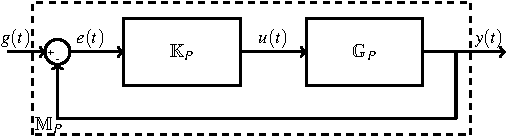
\includegraphics{KpGp.pdf}
	\end{figure}
	\\
	The performance of this setup is improved by providing the reference signal $g(t)$ using an MPC controller in an outer loop. The objective of the MPC controller is to make the output signal $y(t)$ track the reference $r(t)$, while satisfying constraints on the plant output $y(t)$ and input $u(t)$. This is achieved by considering the closed-loop plant model $\mathbb{M}_P$ for the state propagation equation, and an augmented model with $[y(t),u(t)]$ as the output equation. This augmented state-space model is called $\mathbb{M}'_P$.
	\begin{equation*}
	\begin{matrix}
	\zeta(t+1) = A_\zeta\zeta(t) + B_\zeta g(t)\\
	\begin{bmatrix}y(t)\\u(t)\end{bmatrix} = C_\zeta\zeta(t) + \begin{bmatrix}0\\D_\zeta\end{bmatrix}g(t)
	\end{matrix}
	\end{equation*}
	\\
	The optimization problem solved by the MPC at each time step $t$ for a horizon of $N_P$ timesteps is shown below. The lower and upper bounds on $y(t)$ and $u(t)$ are $[y_{min},y_{max}]$ and $[u_{min},u_{max}]$ respectively.
	\begin{equation*}
	\begin{aligned}
	& \underset{\{g(t+k)\}_{k=1}^{N_P}}{\text{min}}
	& & Q_y\mathlarger{\sum\limits_{k=1}^{N_P}}(y(t+k|t)-r(t+k))^2 + Q_{\epsilon}\epsilon^2 \\
	& \text{subject to}
	& & 
	\begin{matrix}
	\zeta(t+k+1) = A_\zeta\zeta(t+k) + B_\zeta g(t+k)\\
	\begin{bmatrix}y(t+k)\\u(t+k)\end{bmatrix} = C_\zeta\zeta(t+k) + \begin{bmatrix}0\\D_\zeta\end{bmatrix}g(t+k)\\
	y_{min}-V_y\epsilon \leq y(t+k) \leq y_{max}+V_y\epsilon \\
	u_{min}-V_u\epsilon \leq u(t+k) \leq u_{max}+V_u\epsilon \\
	\zeta(t|t) = \zeta(t)
	\end{matrix}
	\end{aligned}
	\end{equation*}
	\\
	The quantities $V_y$ and $V_u$ in the MPC formulation are used to avoid infeasibility of the optimization problem over successive iterations, since the reference model $\mathbb{M}'_P$ might not accurately capture the dynamics of the unknown plant $\mathbb{G}_P$. This implies that constraint satisfaction is not guaranteed by the proposed formulation. 
	
	\section{Disturbance sensor}
	In order to improve prediction of closed loop performance, a disturbance sensor $\mathbb{D}$ is designed. The disturbance sensor is a dynamical system whose output is the discrepancy between output of the actual closed loop system  $\mathbb{K}_P$-$\mathbb{G}_P$ and reference closed loop system $\mathbb{M}_P$. The system consists of a deterministic part and a stochastic part, as seen in Fig. \ref{Appended}.
	\begin{figure}[h]
		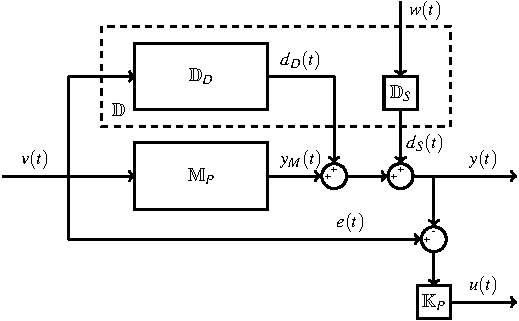
\includegraphics{Mp-D-E.pdf}
		\caption{Reference model appended with disturbance sensor}
		\label{Appended}
	\end{figure}
	\\
	This can be seen as a 2-input 2-output system, whose transfer function is described as
	\begin{equation}
	\begin{bmatrix}
		Y(z) \\ U(z)
	 \end{bmatrix} = 
	 \begin{bmatrix} 
	 \mathbb{M}_P+\mathbb{D}_D & \mathbb{D}_S \\
	 \mathbb{K}_P(I-(\mathbb{M}_P+\mathbb{D}_D)) &  -\mathbb{K}_P\mathbb{D}_S
	 \end{bmatrix}
	 \begin{bmatrix}
	 G(z) \\ W(z)
	 \end{bmatrix}
	\end{equation}
	Note that the dependence of transfer functions on time shift operator $z$ (or $q^{-1}$) is not denoted for ease of notation. The signal $w(t)$ is interpreted as an external noise signal. 
	Since this model represents the closed loop behavior of the system, new closed loop measurements are required to estimate the parameters of the disturbance sensor. These are obtained by performing experiments with excitaion signals $\hat{g}(t)$ on the closed loop model and plant, and measuring the outputs $\hat{y}_M(t)$ and $\hat{y}(t)$ respectively. The output is captured as the data sequence $\hat{D}_{N}=\{\hat{g}(t),\hat{y}_M(t),\hat{y}(t);t\in{1,...,N}\}$.
	The disturbance sensor $\mathbb{D}$ is parameterized as $A_D(q^{-1})y_D(t) = B_D(q^{-1})g(t)+w(t)$, where 
	\begin{equation*}
	\begin{matrix}
	y_D(t) = y(t) - y_M(t) = d_D(t)+d_S(t) \\ 
	A_D(q^{-1}) = 1+\mathlarger{\sum\limits_{i=1}^{n_{a_D}}}a_i^Dq^{-i}\\
	B_D(q^{-1}) = \mathlarger{\sum\limits_{i=1}^{n_{b_D}}}b_i^Dq^{-i}
	\end{matrix}  
	\end{equation*}
	Using standard ARX identification, the coefficients $a_i^D$ and $b_i^D$ are estimated by solving the optimization problem
	\begin{equation*}
	\begin{aligned}
	& \underset{a_i^D,b_i^D}{\text{min}}
	& & \frac{1}{N}\mathlarger{\sum\limits_{t=1}^N}\mathlarger{\mathlarger{|}}A_D(q^{-1})(\hat{y}(t)-\hat{y}_M(t))-B_K(q^{-1})(\hat{g}(t))\mathlarger{\mathlarger{|}}^2 \\
	\end{aligned}
	\end{equation*}
	
	  
\end{enumerate} 

	
                                                              




\begin{thebibliography}{99}

\bibitem{c1} G. O. Young, �Synthetic structure of industrial plastics (Book style with paper title and editor),� 	in Plastics, 2nd ed. vol. 3, J. Peters, Ed.  New York: McGraw-Hill, 1964, pp. 15�64.
\bibitem{c2} W.-K. Chen, Linear Networks and Systems (Book style).	Belmont, CA: Wadsworth, 1993, pp. 123�135.
\bibitem{c3} H. Poor, An Introduction to Signal Detection and Estimation.   New York: Springer-Verlag, 1985, ch. 4.
\bibitem{c4} B. Smith, �An approach to graphs of linear forms (Unpublished work style),� unpublished.
\bibitem{c5} E. H. Miller, �A note on reflector arrays (Periodical style�Accepted for publication),� IEEE Trans. Antennas Propagat., to be publised.
\bibitem{c6} J. Wang, �Fundamentals of erbium-doped fiber amplifiers arrays (Periodical style�Submitted for publication),� IEEE J. Quantum Electron., submitted for publication.
\bibitem{c7} C. J. Kaufman, Rocky Mountain Research Lab., Boulder, CO, private communication, May 1995.
\bibitem{c8} Y. Yorozu, M. Hirano, K. Oka, and Y. Tagawa, �Electron spectroscopy studies on magneto-optical media and plastic substrate interfaces(Translation Journals style),� IEEE Transl. J. Magn.Jpn., vol. 2, Aug. 1987, pp. 740�741 [Dig. 9th Annu. Conf. Magnetics Japan, 1982, p. 301].
\bibitem{c9} M. Young, The Techincal Writers Handbook.  Mill Valley, CA: University Science, 1989.
\bibitem{c10} J. U. Duncombe, �Infrared navigation�Part I: An assessment of feasibility (Periodical style),� IEEE Trans. Electron Devices, vol. ED-11, pp. 34�39, Jan. 1959.
\bibitem{c11} S. Chen, B. Mulgrew, and P. M. Grant, �A clustering technique for digital communications channel equalization using radial basis function networks,� IEEE Trans. Neural Networks, vol. 4, pp. 570�578, July 1993.
\bibitem{c12} R. W. Lucky, �Automatic equalization for digital communication,� Bell Syst. Tech. J., vol. 44, no. 4, pp. 547�588, Apr. 1965.
\bibitem{c13} S. P. Bingulac, �On the compatibility of adaptive controllers (Published Conference Proceedings style),� in Proc. 4th Annu. Allerton Conf. Circuits and Systems Theory, New York, 1994, pp. 8�16.
\bibitem{c14} G. R. Faulhaber, �Design of service systems with priority reservation,� in Conf. Rec. 1995 IEEE Int. Conf. Communications, pp. 3�8.
\bibitem{c15} W. D. Doyle, �Magnetization reversal in films with biaxial anisotropy,� in 1987 Proc. INTERMAG Conf., pp. 2.2-1�2.2-6.
\bibitem{c16} G. W. Juette and L. E. Zeffanella, �Radio noise currents n short sections on bundle conductors (Presented Conference Paper style),� presented at the IEEE Summer power Meeting, Dallas, TX, June 22�27, 1990, Paper 90 SM 690-0 PWRS.
\bibitem{c17} J. G. Kreifeldt, �An analysis of surface-detected EMG as an amplitude-modulated noise,� presented at the 1989 Int. Conf. Medicine and Biological Engineering, Chicago, IL.
\bibitem{c18} J. Williams, �Narrow-band analyzer (Thesis or Dissertation style),� Ph.D. dissertation, Dept. Elect. Eng., Harvard Univ., Cambridge, MA, 1993. 
\bibitem{c19} N. Kawasaki, �Parametric study of thermal and chemical nonequilibrium nozzle flow,� M.S. thesis, Dept. Electron. Eng., Osaka Univ., Osaka, Japan, 1993.
\bibitem{c20} J. P. Wilkinson, �Nonlinear resonant circuit devices (Patent style),� U.S. Patent 3 624 12, July 16, 1990. 






\end{thebibliography}




\end{document}
